\documentclass[thesis.tex]{subfiles}

\chapter{Cơ sở lý thuyết}
Chương 2 trình bày cơ sở lý thuyết về học máy, học sâu cùng \TODO{...}.

\section{Học máy}

\subsection{Tổng quan về học máy}

Học máy (Machine learning - ML) là một nhánh con của trí tuệ nhân tạo. Nghiên cứu học máy tập trung phát triển và xây dựng các thuật toán và kỹ thuật để giúp chương trình máy tính có thể "học" thi thực một tác nào đó từ kinh nghiệm. Trong \cite{mitchell1997machine}, nhà tiên phong về học máy Tom M. Mitchell định nghĩa như sau: Một chương trình máy tính được nói là học từ kinh nghiệm \textit{E} để thực thi một tác vụ \textit{T} nếu khả năng của chương trình được đo bằng độ đo \textit{P} tiến bộ với kinh nghiệm \textit{E}. Rõ ràng hơn, học máy là những chương trình máy tính có thể tự học được dữ liệu mà không cần được lập trình một cách cụ thể.

Với các cách định nghĩa \textit{T}, \textit{P}, và \textit{E} khác nhau, các thuật toán học máy có thể được phân vào các nhóm: học có giám sát, học không giám sát, học bán giám sát, và học tăng cường.

\textbf{Học có giám sát} là lớp các thuật toán sử dụng dữ liệu được gán nhãn từ trước để tìm mối liên hệ giữa đầu vào và đầu ra. Mục tiêu của học có giám sát là tạo ra mô hình có thể dự đoán được đầu ra cho các đầu vào mới mà mô hình chưa gặp bao giờ. Tập dữ liệu gán nhãn trên được gọi là dữ liệu huấn luyện. Cho tập dữ liệu huấn luyện gồm $N$ ví dụ $D = \{(\bm{x}_1, y_1), ..., (\bm{x}_N, y_N)\}$ trong đó $\bm{x}_i$ là vec-tơ đặc trưng của ví dụ tứ $i$ và $y_i$ là nhãn tương ứng. Thuật toán học có giám sát tìm hàm ánh xạ $f: X \longrightarrow Y$ trong đó $X$ là không gian vec-tơ đầu vào và $Y$ là tập các nhãn. 

Các thuật toán học có giảm sát thường được sử dụng để giải quyết hai loại bài toán: phân loại (classification) và hồi quy (regression). Bài toán phân loại có nhãn rời rạc thuộc một tập cho sẵn. Ví dụ: phân loại đồ vật, phân loại phương tiện giao thông, phân loại giới tính dựa trên giọng nói. Khác với bài toán phân loại, bài toán hồi quy lại có nhãn nằm trên một miền liên tục. Ví dụ: dự đoán giá nhà đất, dự đoán thị trường chứng khoán.

Trong \textbf{học không giám sát}, khác với học có giám sát, ta chỉ có dữ liệu đầu vào mà không có dữ liệu đầu ra. Mục tiêu chính của các thuật toán là tìm ra cấu trúc ẩn trong dữ liệu hoặc trích xuất đặc trưng chung của tập dữ liệu.

\textbf{Học bán giám sát} nằm giữa học có giám sát và không có giám sát. Học bán giám sát thường được sử dụng khi có một lượng lớn dữ liệu không có nhãn và một số ít dữ liệu có nhãn. Phương pháp học bán giám sát nổi tiếng nhất - tự huấn luyện (self-training) sử dụng mô hình huấn luyện trên tập có nhãn để sinh nhãn giả từ tập không nhãn nhằm tăng cường khả năng học của mô hình.

Hệ thống \textbf{học củng cố} được xem như là một tác tử trong một môi trường vô định và phức tạp. Với mỗi hành động, tác tử này nhận điểm thưởng hoặc phạt từ môi trường. Mục tiêu của học củng cố là các tác tử thông minh để tối đa điểm thưởng và thực hiện tác vụ của nó. Học củng cố hiện đang là lĩnh vực nghiên cứu tập trung nhiều nguồn lực và công sức với nhiều ứng dụng thực tế liên quan tới điều khiển robot hay vận hành nhà máy một cách tự động.

\subsection{Mạng nơ-ron nhân tạo}
Mạng nơ-ron nhân tạo (Artificial neural networks - ANN) là một mô hình tính toán mô phỏng cách nơ-ron trong não người phân tích và xử lý thông tin. Học sâu với nền tảng là ANN cho phép xử lý dữ liệu và thông tin với độ chính xác vượt xa các mô hình xác suất cổ điển và tốc độ vượt trội so với con người. 

\begin{figure}[h]
  \centering
  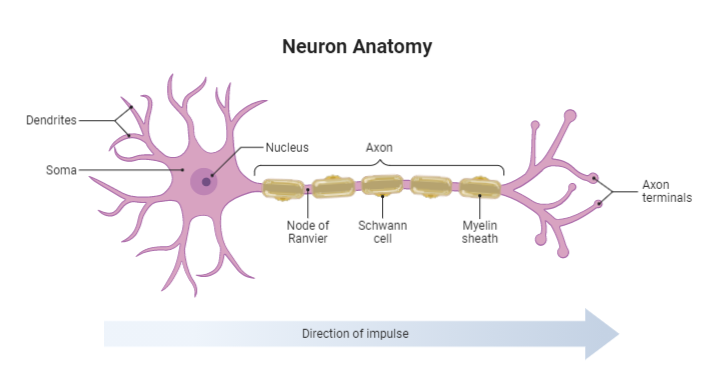
\includegraphics[width=0.9\textwidth]{images/neuron.png}
  \caption{Cấu tạo nơ-ron sinh học \protect\footnotemark}
  \label{fig:neuron}
\end{figure}
\footnotetext{https://app.biorender.com/biorender-templates/t-5f5b7e6139954000b2bde860-neuron-anatomy}

Nơ-ron sinh học gồm 3 phần chính: dendrite, thân tế bào (soma) và axon (Hình \ref*{fig:neuron}). Đầu tiên, tín hiệu đầu vào được thu thập bởi các khớp thần kinh của dendrite. Vai trò của soma là xử lý đầu vào và tổng hợp thông tin dựa vào độ quan trọng của tín hiệu. Sau đó, axon sẽ truyền thông tin đã được xử lý tới đầu ra. Thành phần cấu thành nên ANN là perceptron cũng có cách thức hoạt động tương tự. Perceptron bao gồm lớp đầu vào, tập trọng số cùng hàm kích hoạt để tổng hợp thông tin và lớp đầu ra, tương tự như dendrite, soma và axon.

Mạng nơ-ron là mô hình gồm nhiều lớp chồng lên nhau, mỗi lớp bao gồm nhiều perceptron (hay nơ-ron) tổng hợp thông tin từ lớp trước, mỗi lớp có một tập các nơ-ron độc lập. Lớp đầu tiên trong mạng được gọi là lớp đầu vào (input layer), lớp cuối cùng được gọi là lớp đầu ra (output layer), các lớp ở giữa được gọi là lớp ẩn (hidden layer) (Hình \ref{fig:neuron}). 

\begin{figure}[h]
  \centering
  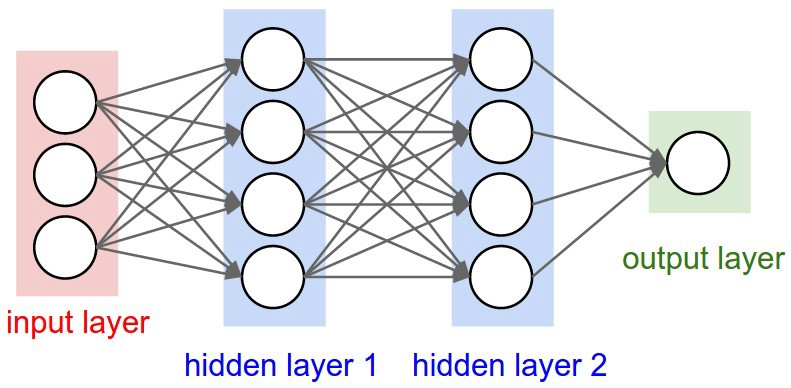
\includegraphics[width=0.8\textwidth]{images/artificial-neural-network.jpeg}
  \caption{Cấu trúc của mạng nơ-ron nhân tạo\protect\footnotemark}
  \label{fig:neuron}
\end{figure}
\footnotetext{https://towardsdatascience.com/vanilla-neural-networks-in-r-43b028f415}

Cho một mạng nơ-ron nhân tạo gồm $L$ lớp, với $\bm{a}^i$ là tập các nơ-ron trong lớp thứ $i$, hai lớp nơ-ron liên tiếp có chỉ số $i$ và $i+1$ được kết nối với nhau bằng một ma trận trọng số $\bm{W}^i$ và một vec-tơ bias $\bm{b}^i$. Ta có thể mô tả quá trình tính toán các nơ-ron từ lớp đầu vào và đầu ra dưới dạng toán học như sau:

\begin{equation}
  \bm{a}^{(i)} = \sigma(\bm{W}^i\bm{a}^{(i-1)} + \bm{b}^i),\ 0 \le i \le L 
\end{equation}

Trong đó, $\sigma$ được gọi là hàm kích hoạt (activation function). Hàm kích hoạt là một thành phần quan trọng không thể thiếu trong mạng nơ-ron nhân tạo. Để mạng nơ-ron nhân tạo có thể xấp xỉ hay học được những biến đổi phức tạp, $\sigma$ phải là một hàm phi tuyến. Nếu không có hàm kích hoạt hay hàm kích hoạt là tuyến tính thì mạng nơ-ron dù có nhiều lớp đến đâu cũng có thể quy về một hàm tuyến tính và không có khả năng học được nhiều thông tin từ dữ liệu.

Có rất nhiều hàm kích hoạt khác nhau, ví dụ như hàm ReLU, hàm sigmoid, hàm Tanh, hàm softplus,... Trong các mạng nơ-ron hiện đại, hàm ReLU \cite{nair2010rectified} được sử dụng phổ biến nhất do có nhiều lợi ích cho quá trình huấn luyện và tốc độ tính toán nhanh:

\begin{equation}
  ReLU(x)=\max (0, x)
\end{equation}

Quá trình lần lượt tính toán mạng nơ-ron từ lớp đầu vào, tới lớp ẩn và cuối cùng là lớp đầu ra được gọi là quá trình lan truyền tiến (feedforward). 

Mạng nơ-ron học từ quá trình đối nghịch với lan truyền tiến gọi là lan truyền ngược (backpropagation). Với vec-tơ đặc trung đầu vào $\bm{x}$ với nhãn tương ứng $y$, đầu tiên ta tính giá trị của nơ-ron lớp đầu ra $\bm{a}^{L-1}$ bằng quá trình lan truyền tiến. Sau đó, ta "lan truyền" sai khác giữa $\bm{a}^{L-1}$ và $y$ tới toàn mạng để điều chỉnh các bộ tham số $\bm{W}^i$ và $\bm{b}^i$ với mục tiêu để giảm sai khác này.

Để đo đạc sự sai khác trong đầu ra của mạng và nhãn đầu vào, ta sử dụng một hàm mất mát. Dựa vào tác vụ khác nhau của bài toán ta cần sử dụng các hàm mất mát khác nhau. Thông thường, bài toán hồi quy sử dụng hàm trung bình bình phương sai số (mean square error - MSE), còn bài toán phân loại sử dụng hàm entropy chéo (cross entropy - CE). Với tập dữ liệu $D = \{(\bm{x}_1, y_1), ..., (\bm{x}_N, y_N)\}$, giả sử lớp cuối cùng của mạng có một nơ-ron, gọi $a^{L-1}_i$ là giá trị của nơ-ron đầu ra tương ứng với dữ liệu đầu vào $\bm{x}_i$. Hàm mất mát MSE được tính như sau:

\begin{equation}
  MSE = \dfrac{1}{N} \sum_{i=1}^N (y_i - a^{L-1}_i)^2
\end{equation}

hàm CE được tính theo công thức:

\begin{equation}
  CE = -\dfrac{1}{N} \sum_{i=1}^N a^{L-1}_i log(y_i)
\end{equation}

Để điều chỉnh các tham số, ta cần phải biết giá trị cập nhật cho mỗi tham số. Dựa trên giá trị mất mát, các tín hiệu mất mát của nơ-ron trong lớp thứ $i$ được tính toán dựa trên lỗi mà lớp thứ $i+1$ gây ra. Tín hiệu mất mát này được lan truyền từ lớp đầu ra về tới lớp đầu vào, sau đó thực hiện cập nhật các tham số $\bm{W}, \bm{b}$ nhằm giảm các giá trị lỗi. Các giá trị lỗi của các bộ tham số được gọi là gradient. 

Sau khi có bộ gradient, ta có thể cập nhật mạng bằng cách đi ngược lại với hướng của gradient. Giá trị mất mát trên bộ dữ liệu sẽ giảm nếu gradient được cập nhật với bước đủ nhỏ. Bằng cách lặp đi lặp lại quá trình lan truyền tiến, lan truyền ngược và cập nhật tham số bằng gradient, bộ tham số có thể hội tụ tại một điểm cực tiểu của hàm mất mát. Phương pháp tối ưu lặp này được gọi là gradient descent (Hình \ref*{fig:gradient-descent}).

\begin{figure}[h]
  \centering
  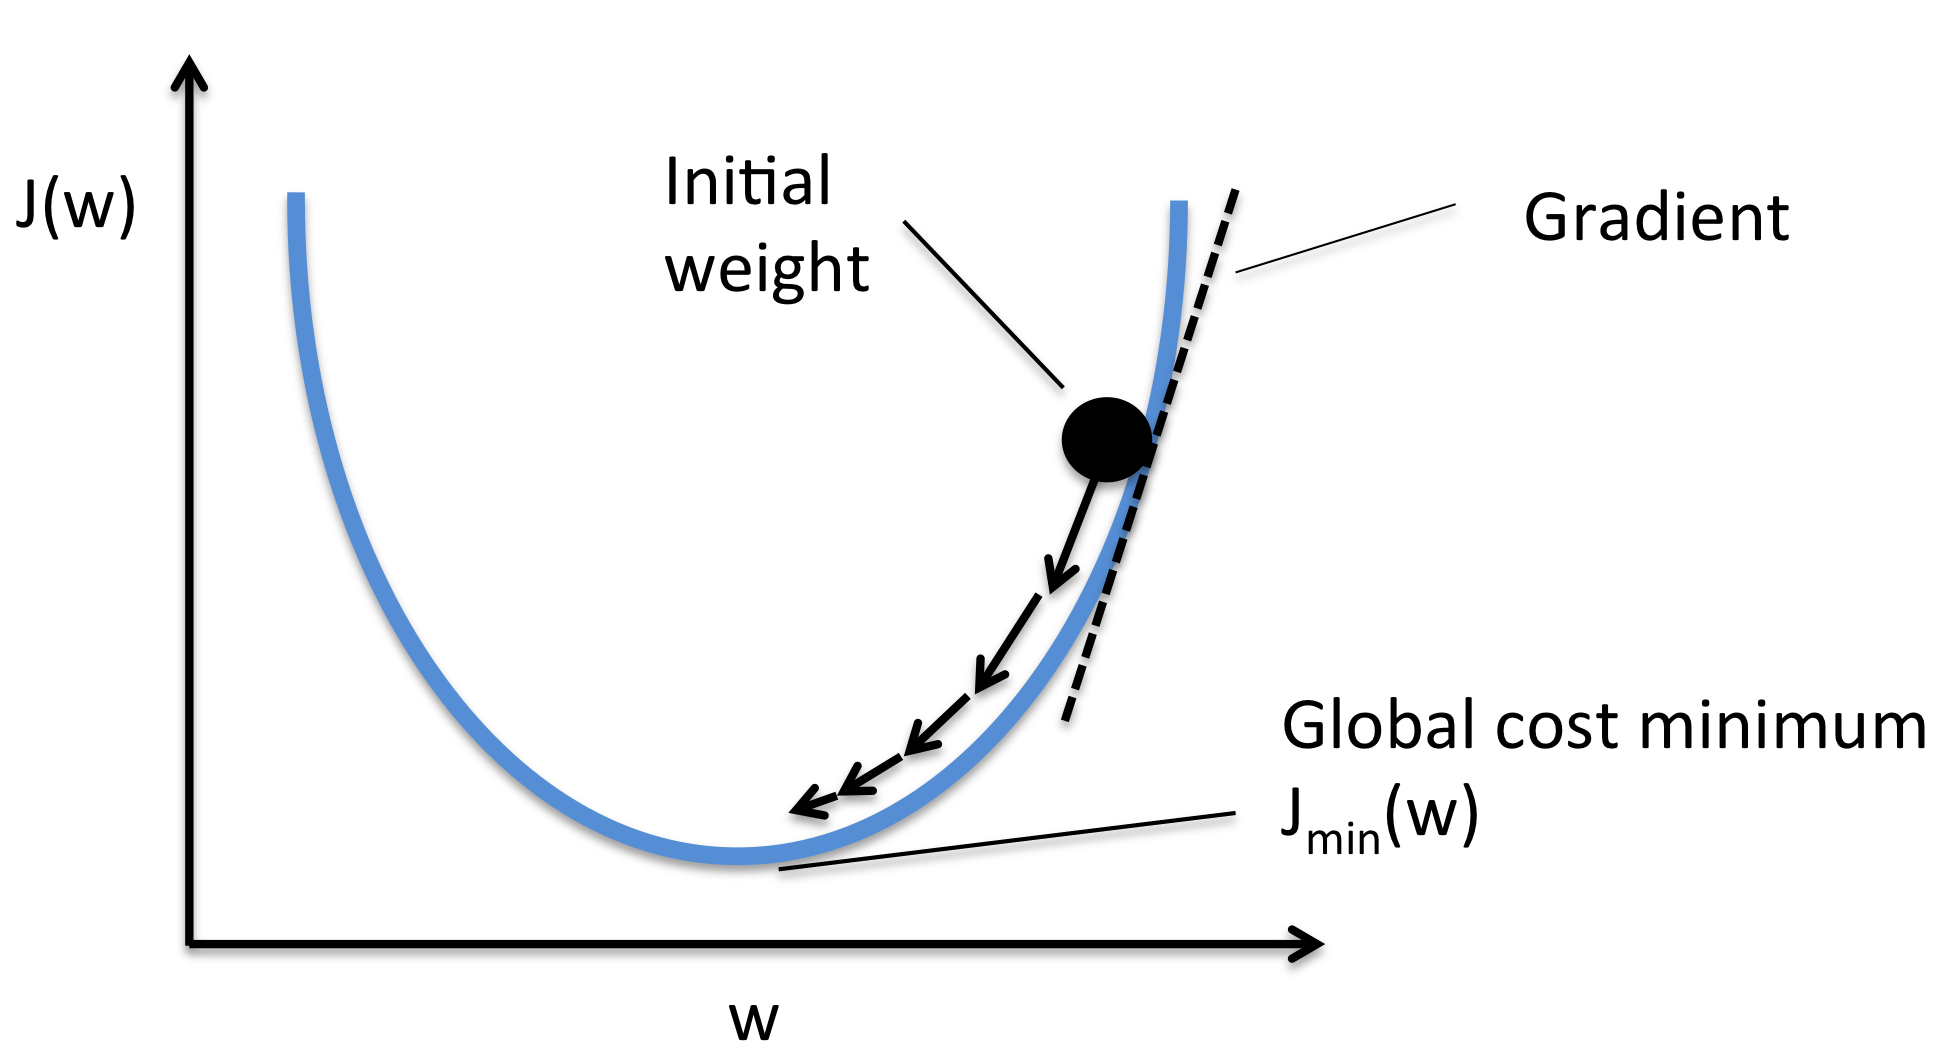
\includegraphics[width=0.8\textwidth]{images/gradient-descent.png}
  \caption{Phương pháp gradient descent \protect\footnotemark}
  \label{fig:gradient-descent}
\end{figure}
\footnotetext{https://machinelearningnotepad.wordpress.com/2018/04/15/gradient-descent}

Hệ số học (learning rate) được điều chỉnh để kiểm soát bước cập nhật trong gradient descent. Với hệ số học lớn, bước đi của gradient descent trở nên lớn hơn và có thể gặp khó khăn hội tụ khi gần điểm cực tiểu. Hệ số học nhỏ hơn giúp mô hình dễ hội tụ hơn tuy nhiên mất nhiều vòng lặp hơn. 

Phương pháp gradient descent truyền thống sử dụng gradient cho cả bộ dữ liệu. Tuy vậy, với các bộ dữ liệu cực lớn, điều này là không thể. Do vậy, ta phải xấp xỉ gradient của cả bộ dữ liệu bằng cách chia nhỏ bộ dữ liệu gốc thành các lô nhỏ (mini-batch) và thực hiện việc cập nhật trọng số trên các lô này. Phương pháp xấp xỉ này được gọi là stochastic gradient descent - SGD. Gần đây, nhiều phương pháp biến thể của SGD được phát triển có thể kể đến như RMSprop, Adadelta \cite{zeiler2012adadelta} và Adam \cite{kingma2014adam} giúp tăng tốc độ hội tụ cũng như tăng cường hiệu năng khi huấn luyện mô hình.

\section{Học sâu}

Học sâu là một lớp các mô hình học máy được xây dựng dựa trên mạng nơ-ron nhân tạo. Nếu mạng nơ-ron nhân tạo chỉ gồm vài lớp nơ-ron, các mạng học sâu được thiết kế để mở rộng ra hàng chục, trăm, thậm chí hàng nghìn lớp nơ-ron. Điều này giúp các mô hình học sâu giải quyết được nhiều bài toán phức tạp với độ chính xác ngang bằng con người. Huấn luyện mô hình học sâu yêu cầu một lượng dữ liệu lớn và tài nguyên tính toán lớn. Trong thập kỉ vừa qua với sự bùng nổ của dữ liệu và tài nguyên tính toán, nghiên cứu học sâu trở thành tâm điểm của lĩnh vực trí tuệ nhân tạo.

\subsection{Mạng nơ-ron tích chập}

Mạng nơ-ron tích chập (Convolutional neural networks), hay mạng tích chập, được đề xuất lần đầu vào năm 1989 bởi Yan LeCun \cite{lecun1989backpropagation} để giải quyết bài toán nhận dạng chữ viết tay. Mạng tích chập được thiết kế với mục tiêu xử lý dữ liệu dạng bảng - lưới, ví dụ như dữ liệu chuỗi thời gian có thể biểu diễn dưới dạng bảng 1D hay ảnh là dữ liệu 2D của các điểm ảnh. Năm 2012, Alex Krizhevsky xây dựng một mạng tích chập (AlexNet \cite{krizhevsky2012imagenet}) và tăng tốc quá trình huấn luyện sử dụng GPU. Mô hình đề xuất của Krizhevsky đứng đầu trong bảng xếp hạng trong cuộc thi phân loại ảnh ImageNet \cite{deng2009imagenet} với độ chính xác vượt hơn 10\% các đội tham gia. Hiện nay, mạng tích chập được áp dụng xử lý nhiều bài toán phức tạp trong xử lý ảnh, xử lý ngôn ngữ tự nhiên, xử lý tín hiệu âm thanh, ...

\begin{figure}[h]
  \centering
  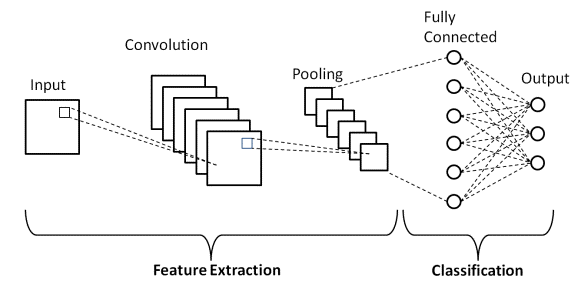
\includegraphics[width=0.8\textwidth]{images/convnet.png}
  \caption{Các thành phần cơ bản của mạng tích chập \protect\footnotemark}
  \label{fig:convnet}
\end{figure}
\footnotetext{https://www.upgrad.com/blog/basic-cnn-architecture}

Thời điểm hiện tại đã có rất nhiều kiến trúc mạng nơ-ron tích chập khác nhau được xây dựng, tuy nhiên chúng đều được cấu thành từ các lớp thành phần (Hình \ref{fig:convnet}), bao gồm: lớp tích chập (convolutional layer), lớp tổng hợp (pooling layer) và lớp kết nối đầy đủ (fully connected layer).

\subsubsection{Lớp tích chập}
Lớp tích chập là lớp được sử dụng nhiều nhất trong mạng nơ-ron tích chập, mục tiêu của lớp tích chập là học các đặc trưng cục bộ từ dữ liệu đầu vào (Hình \ref{fig:convolutional-feature}). Cái tên lớp tích chập xuất phát từ việc lớp sử dụng phép biến đổi toán học tuyến tính gọi là tích chập (convolution).

\begin{figure}[h]
  \centering
  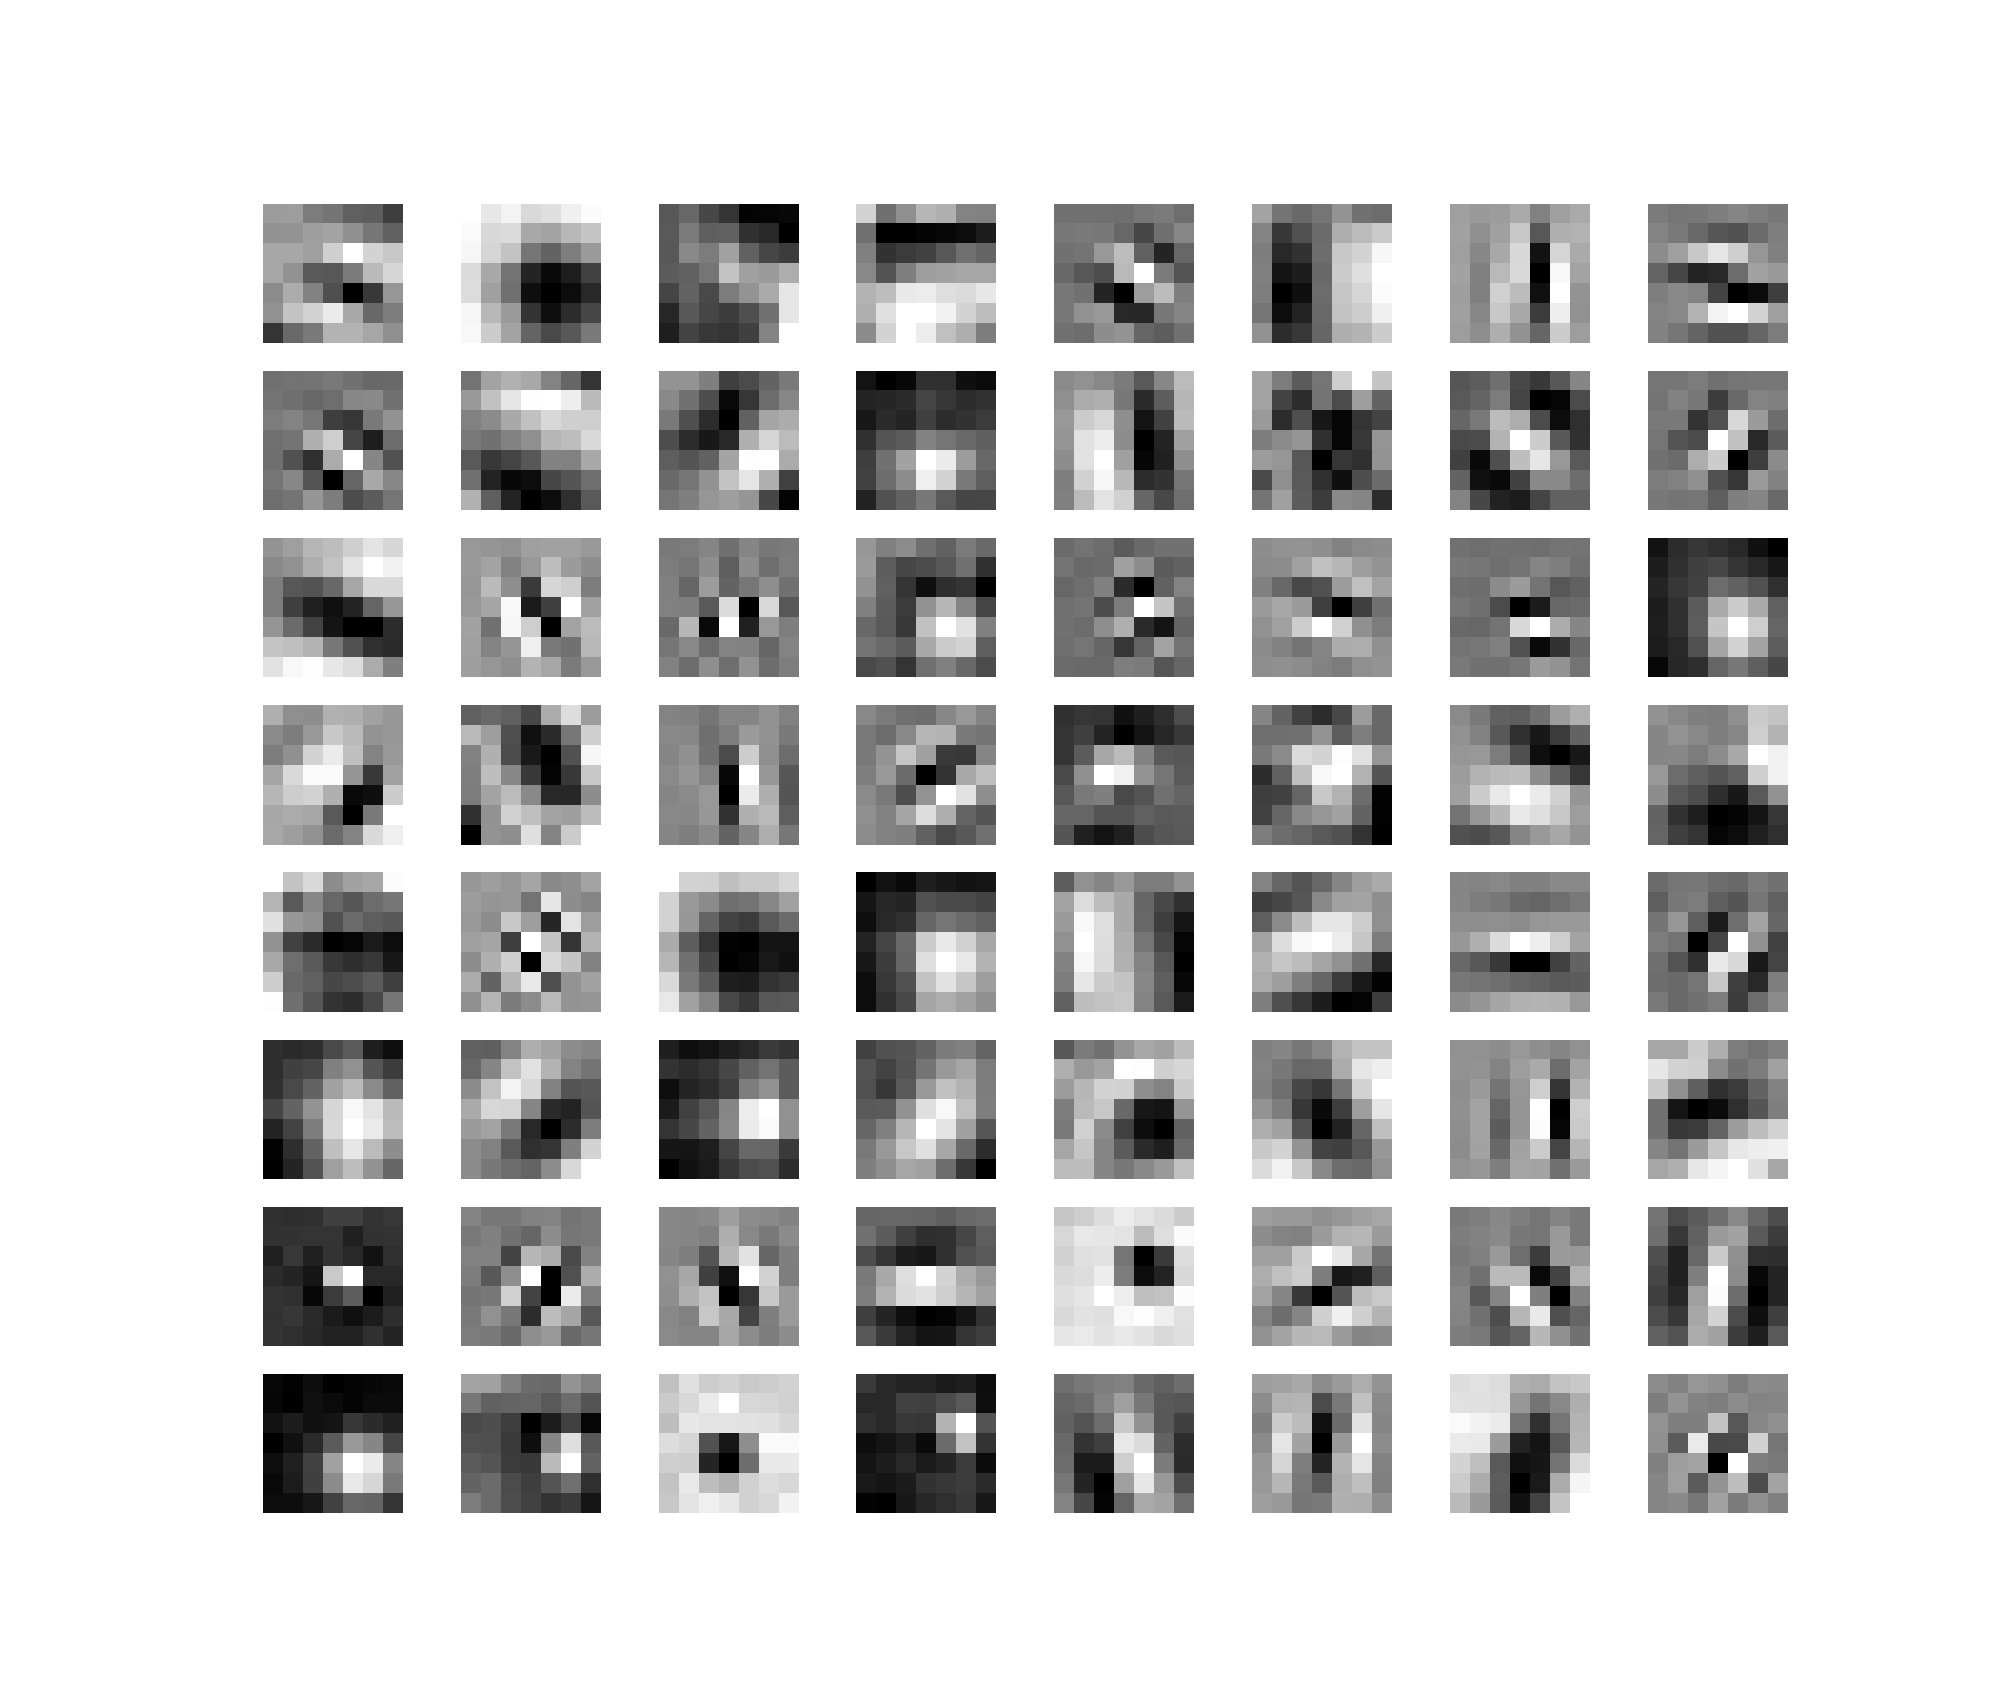
\includegraphics[width=0.7\textwidth]{images/convolutional-feature.png}
  \caption{Các đặc trưng học được trong lớp tích chập \protect\footnotemark}
  \label{fig:convolutional-feature}
\end{figure}
\footnotetext{https://debuggercafe.com/visualizing-filters-and-feature-maps-in-convolutional-neural-networks-using-pytorch}

Ban đầu, phép tích chập được được sử dụng phổ biến trong xử lý tín hiệu. Về sau nguyên lý biến đổi trong tích chập mới được áp dụng trong lĩnh vực xử lý hình ảnh. Công thức tích chập 

\subsubsection{Lớp tổng hợp}
\subsubsection{Lớp kết nối đầy đủ}


\section{Metric Learning}
\subsection{Contrastive loss}
\subsection{Triplet loss}

\section{Trích xuất thông tin}
Xử lý tín hiệu đóng vai trò quan trọng trong bất kì hệ thống tiếng nói nào, từ nhận dạng tiếng nói tới nhận dạng người nói. Hai trong những đặc trưng âm thanh phổ biến nhất được sử dụng là filter banks và Mel-Frequency Cepstral Coefficients (MFCCs). 

Trích xuất filter banks và MFCCs tuân theo quy trình khá tương tự nhau, tính toán filter banks yêu cầu ít hơn MFCCs một số bước. Quy trình trích xuất MFCCs gồm 6 bước chính (Hình \ref{fig:mfcc-computation}): nhấn mạnh (pre-emhphasis), cắt khung (framing), cửa sổ (windowing), biến đổi Fourier (Fourier transform), filter bank và cuối cùng là biến đổi cô sin rời rạc (Discrete cosine transform) để có kết quả là MFCC.
% https://haythamfayek.com/2016/04/21/speech-processing-for-machine-learning.html
\subsubsection{Bước 1: Nhấn mạnh}

Trong bước này, tín hiệu đầu vào được đưa qua một bộ lọc để khuếch đại các tín hiệu với tần số cao. Tín hiệu đầu ra của bộ lọc $y_t$ tại thời gian $t$ được tính như sau: 

\begin{equation}
  y_t = x_y - \alpha x_{t-1} 
\end{equation}

Trong đó, $x$ là dãy tín hiệu đầu vào và $\alpha$ là hệ số của bộ lọc. $\alpha$ thường nhận giá trị $0.95$ hoặc $0.97$.

\subsubsection{Bước 2: Cắt khung}

\subsubsection{Bước 3: Nhấn mạnh}

\subsubsection{Bước 4: Nhấn mạnh}

\subsubsection{Bước 5: Nhấn mạnh}

\subsubsection{Bước 6: Nhấn mạnh}

\begin{figure}[h]
  \centering
  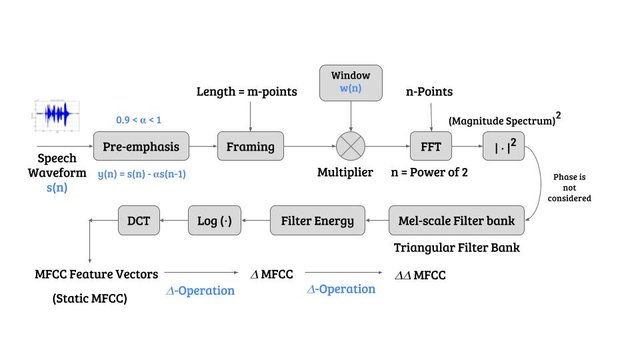
\includegraphics[width=0.9\textwidth]{images/mfcc-computation.jpg}
  \caption{Thuật toán trich xuất MFCCs \cite{barai2017asr}}
  \label{fig:mfcc-computation}
\end{figure}